\documentclass[]{achemso}
\usepackage{lmodern}
\usepackage{amssymb,amsmath}
\usepackage{ifxetex,ifluatex}
\usepackage{fixltx2e} % provides \textsubscript
\ifnum 0\ifxetex 1\fi\ifluatex 1\fi=0 % if pdftex
  \usepackage[T1]{fontenc}
  \usepackage[utf8]{inputenc}
\else % if luatex or xelatex
  \ifxetex
    \usepackage{mathspec}
  \else
    \usepackage{fontspec}
  \fi
  \defaultfontfeatures{Ligatures=TeX,Scale=MatchLowercase}
\fi
% use upquote if available, for straight quotes in verbatim environments
\IfFileExists{upquote.sty}{\usepackage{upquote}}{}
% use microtype if available
\IfFileExists{microtype.sty}{%
\usepackage{microtype}
\UseMicrotypeSet[protrusion]{basicmath} % disable protrusion for tt fonts
}{}
\usepackage[unicode=true]{hyperref}
\PassOptionsToPackage{usenames,dvipsnames}{color} % color is loaded by hyperref
\hypersetup{
            pdftitle={Modeling Chronic Toxicity: A comparison of experimental variability with (Q)SAR/read-across predictions},
            pdfauthor={Christoph Helma1; David Vorgrimmler1; Denis Gebele1; Martin Gütlein2; Barbara Engeli3; Jürg Zarn3; Benoit Schilter4; Elena Lo Piparo4},
            pdfkeywords={(Q)SAR, read-across, LOAEL, experimental variability},
            colorlinks=true,
            linkcolor=Maroon,
            citecolor=Blue,
            urlcolor=Blue,
            breaklinks=true}
\urlstyle{same}  % don't use monospace font for urls
\usepackage{longtable,booktabs}
% Fix footnotes in tables (requires footnote package)
\IfFileExists{footnote.sty}{\usepackage{footnote}\makesavenoteenv{long table}}{}
\usepackage{graphicx,grffile}
\makeatletter
\def\maxwidth{\ifdim\Gin@nat@width>\linewidth\linewidth\else\Gin@nat@width\fi}
\def\maxheight{\ifdim\Gin@nat@height>\textheight\textheight\else\Gin@nat@height\fi}
\makeatother
% Scale images if necessary, so that they will not overflow the page
% margins by default, and it is still possible to overwrite the defaults
% using explicit options in \includegraphics[width, height, ...]{}
\setkeys{Gin}{width=\maxwidth,height=\maxheight,keepaspectratio}
\IfFileExists{parskip.sty}{%
\usepackage{parskip}
}{% else
\setlength{\parindent}{0pt}
\setlength{\parskip}{6pt plus 2pt minus 1pt}
}
\setlength{\emergencystretch}{3em}  % prevent overfull lines
\providecommand{\tightlist}{%
  \setlength{\itemsep}{0pt}\setlength{\parskip}{0pt}}
\setcounter{secnumdepth}{0}
% Redefines (sub)paragraphs to behave more like sections
\ifx\paragraph\undefined\else
\let\oldparagraph\paragraph
\renewcommand{\paragraph}[1]{\oldparagraph{#1}\mbox{}}
\fi
\ifx\subparagraph\undefined\else
\let\oldsubparagraph\subparagraph
\renewcommand{\subparagraph}[1]{\oldsubparagraph{#1}\mbox{}}
\fi

% set default figure placement to htbp
\makeatletter
\def\fps@figure{htbp}
\makeatother

\usepackage{a4wide}
\linespread{2}
\usepackage{lineno}
\linenumbers
\usepackage{subfig}
\AtBeginDocument{%
\renewcommand*\figurename{Figure}
\renewcommand*\tablename{Table}
}
\AtBeginDocument{%
\renewcommand*\listfigurename{List of Figures}
\renewcommand*\listtablename{List of Tables}
}
\usepackage{float}
\floatstyle{ruled}
\makeatletter
\@ifundefined{c@chapter}{\newfloat{codelisting}{h}{lop}}{\newfloat{codelisting}{h}{lop}[chapter]}
\makeatother
\floatname{codelisting}{Listing}
\newcommand*\listoflistings{\listof{codelisting}{List of Listings}}

\title{Modeling Chronic Toxicity: A comparison of experimental variability with
(Q)SAR/read-across predictions}
\author{Christoph Helma\textsuperscript{1} \and David Vorgrimmler\textsuperscript{1} \and Denis Gebele\textsuperscript{1} \and Martin Gütlein\textsuperscript{2} \and Barbara Engeli\textsuperscript{3} \and Jürg Zarn\textsuperscript{3} \and Benoit Schilter\textsuperscript{4} \and Elena Lo Piparo\textsuperscript{4}}
\date{\today}

\begin{document}
\maketitle
\begin{abstract}
This study compares the accuracy of (Q)SAR/read-across predictions with
the experimental variability of chronic lowest-observed-adverse-effect
levels (LOAELs) from \emph{in vivo} experiments. We could demonstrate
that predictions of the lazy structure-activity relationships
(\texttt{lazar}) algorithm within the applicability domain of the
training data have the same variability as the experimental training
data. Predictions with a lower similarity threshold (i.e.~a larger
distance from the applicability domain) are also significantly better
than random guessing, but the errors to be expected are higher and a
manual inspection of prediction results is highly recommended.
\end{abstract}

\textsuperscript{1} in silico toxicology gmbh, Basel,
Switzerland\newline\textsuperscript{2} Inst. f. Computer Science,
Johannes Gutenberg Universität Mainz, Germany\newline\textsuperscript{3}
Federal Food Safety and Veterinary Office (FSVO) , Risk Assessment
Division , Bern , Switzerland\newline\textsuperscript{4} Chemical Food
Safety Group, Nestlé Research Center, Lausanne, Switzerland

\section{Introduction}\label{introduction}

Relying on standard animal toxicological testing for chemical hazard
identification and characterization is increasingly questioned on both
scientific and ethical grounds. In addition, it appears obvious that
from a resource perspective, the capacity of standard toxicology to
address the safety of thousands of untested chemicals (Fowler, Savage,
and Mendez 2011) to which human may be exposed is very limited. It has
also been recognized that getting rapid insight on toxicity of chemicals
in case of emergency safety incidents or for early prioritization in
research and development (safety by design) is a big challenge mainly
because of the time and cost constraints associated with the generation
of relevant animal data. In this context, alternative approaches to
obtain timely and fit-for-purpose toxicological information are being
developed. Amongst others \emph{in silico} toxicology methods are
considered highly promising. Importantly, they are raising more and more
interests and getting increased acceptance in various regulatory (e.g.
(ECHA 2008, EFSA (2016), EFSA (2014), Health Canada (2016), OECD
(2015))) and industrial (e.g. (Stanton and Krusezewski 2016, Lo Piparo
et al. (2011))) frameworks.

For a long time already, computational methods have been an integral
part of pharmaceutical discovery pipelines, while in chemical food
safety their actual potentials emerged only recently (Lo Piparo et al.
2011). In this field, an application considered critical is in the
establishment of levels of safety concern in order to rapidly and
efficiently manage toxicologically uncharacterized chemicals identified
in food. This requires a risk-based approach to benchmark exposure with
a quantitative value of toxicity relevant for risk assessment (Schilter
et al. 2014). Since chronic studies have the highest power (more animals
per group and more endpoints than other studies) and because long-term
toxicity studies are often the most sensitive in food toxicology
databases, predicting chronic toxicity is of prime importance. Up to
now, read-across and Quantitative Structure Activity Relationships
(QSAR) have been the most used \emph{in silico} approaches to obtain
quantitative predictions of chronic toxicity.

The quality and reproducibility of (Q)SAR and read-across predictions
has been a continuous and controversial topic in the toxicological
risk-assessment community. Although model predictions can be validated
with various procedures, to review results in context of experimental
variability has actually been rarely done or attempted. With missing
information about the variability of experimental toxicity data it is
hard to judge the performance of predictive models objectively and it is
tempting for model developers to use aggressive model optimisation
methods that lead to impressive validation results, but also to
overfitted models with little practical relevance.

In the present study, automatic read-across like models were built to
generate quantitative predictions of long-term toxicity. The aim of the
work was not to predict the nature of the toxicological effects of
chemicals, but to obtain quantitative values which could be compared to
exposure. Two databases compiling chronic oral rat Lowest Adverse Effect
Levels (LOAEL) as endpoint were used. An early review of the databases
revealed that many chemicals had at least two independent
studies/LOAELs. These studies were exploited to generate information on
the reproducibility of chronic animal studies and were used to evaluate
prediction performance of the models in the context of experimental
variability.

An important limitation often raised for computational toxicology is the
lack of transparency on published models and consequently on the
difficulty for the scientific community to reproduce and apply them. To
overcome these issues, source code for all programs and libraries and
the data that have been used to generate this manuscript are made
available under GPL3 licenses. Data and compiled programs with all
dependencies for the reproduction of results in this manuscript are
available as a self-contained docker image. All data, tables and figures
in this manuscript was generated directly from experimental results
using the \texttt{R} package \texttt{knitR}.

\section{Materials and Methods}\label{materials-and-methods}

The following sections give a high level overview about algorithms and
datasets used for this study. In order to provide unambiguous references
to algorithms and datasets, links to source code and data sources are
included in the text.

\subsection{Datasets}\label{datasets}

\subsubsection{Nestlé database}\label{nestluxe9-database}

The first database (Nestlé database for further reference) originates
from the publication of (P. Mazzatorta et al. 2008). It contains chronic
(\textgreater{} 180 days) lowest observed effect levels (LOAEL) for rats
(\emph{Rattus norvegicus}) after oral (gavage, diet, drinking water)
administration. The Nestlé database consists of 567 LOAEL values for 445
unique chemical structures. The Nestlé database can be obtained from the
following GitHub links:

\begin{itemize}
\tightlist
\item
  original data:
  \url{https://github.com/opentox/loael-paper/blob/revision/data/LOAEL_mg_corrected_smiles_mmol.csv}
\item
  unique smiles:
  \url{https://github.com/opentox/loael-paper/blob/revision/data/mazzatorta.csv}
\item
  -log10 transfomed LOAEL:
  \url{https://github.com/opentox/loael-paper/blob/revision/data/mazzatorta_log10.csv}.
\end{itemize}

\subsubsection{Swiss Food Safety and Veterinary Office (FSVO)
database}\label{swiss-food-safety-and-veterinary-office-fsvo-database}

Publicly available data from pesticide evaluations of chronic rat
toxicity studies from the European Food Safety Authority (EFSA) (EFSA
2014), the Joint FAO/WHO Meeting on Pesticide Residues (JMPR) (WHO 2011)
and the US EPA (US EPA 2011) were compiled to form the FSVO-database.
Only studies providing both an experimental NOAEL and an experimental
LOAEL were included. The LOAELs were taken as they were reported in the
evaluations. Further details on the database are described elsewhere
(Zarn, Engeli, and Schlatter 2011, Zarn, Engeli, and Schlatter (2013)).
The FSVO-database consists of 493 rat LOAEL values for 381 unique
chemical structures. It can be obtained from the following GitHub links:

\begin{itemize}
\tightlist
\item
  original data:
  \url{https://github.com/opentox/loael-paper/blob/revision/data/NOAEL-LOAEL_SMILES_rat_chron.csv}
\item
  unique smiles and mmol/kg\_bw/day units:
  \url{https://github.com/opentox/loael-paper/blob/revision/data/swiss.csv}
\item
  -log10 transfomed LOAEL:
  \url{https://github.com/opentox/loael-paper/blob/revision/data/swiss_log10.csv}
\end{itemize}

\subsubsection{Preprocessing}\label{preprocessing}

Chemical structures (represented as SMILES (Weininger 1988)) in both
databases were checked for correctness. When syntactically incorrect or
missing SMILES were generated from other identifiers (e.g names, CAS
numbers). Unique smiles from the OpenBabel library (OBoyle et al. 2011)
were used for the identification of duplicated structures.

Studies with undefined or empty LOAEL entries were removed from the
databases. LOAEL values were converted to mmol/kg bw/day units and
rounded to five significant digits. For prediction, validation and
visualisation purposes -log10 transformations are used.

\subsubsection{Derived datasets}\label{derived-datasets}

Two derived datasets were obtained from the original databases:

The
\href{https://github.com/opentox/loael-paper/blob/revision/data/test_log10.csv}{\emph{test}
dataset} contains data from compounds that occur in both databases.
LOAEL values equal at five significant digits were considered as
duplicates originating from the same study/publication and only one
instance was kept in the test dataset. The test dataset has 375 LOAEL
values for 155 unique chemical structures and was used for

\begin{itemize}
\tightlist
\item
  evaluating experimental variability
\item
  comparing model predictions with experimental variability.
\end{itemize}

The
\href{https://github.com/opentox/loael-paper/blob/revision/data/training_log10.csv}{\emph{training}
dataset} is the union of the Nestlé and the FSVO databases and it was
used to build predictive models. LOAEL duplicates were removed using the
same criteria as for the test dataset. The training dataset has 998
LOAEL values for 671 unique chemical structures.

\subsection{Algorithms}\label{algorithms}

In this study we are using the modular lazar (\emph{la}zy
\emph{s}tructure \emph{a}ctivity \emph{r}elationships) framework (A.
Maunz et al. 2013) for model development and validation. The complete
\texttt{lazar} source code can be found on
\href{https://github.com/opentox/lazar/tree/loael-paper.revision}{GitHub}.

lazar follows the following basic
\href{https://github.com/opentox/lazar/blob/loael-paper.revision/lib/model.rb\#L191-L281}{workflow}:

For a given chemical structure lazar

\begin{itemize}
\tightlist
\item
  searches in a database for similar structures (\emph{neighbors}) with
  experimental data,
\item
  builds a local QSAR model with these neighbors and
\item
  uses this model to predict the unknown activity of the query compound.
\end{itemize}

This procedure resembles an automated version of \emph{read across}
predictions in toxicology, in machine learning terms it would be
classified as a \emph{k-nearest-neighbor} algorithm.

Apart from this basic workflow lazar is completely modular and allows
the researcher to use any algorithm for similarity searches and local
QSAR modelling. Algorithms used within this study are described in the
following sections.

\subsubsection{Neighbor identification}\label{neighbor-identification}

Similarity calculations are based on
\href{https://github.com/opentox/lazar/blob/loael-paper.revision/lib/compound.rb\#L38-L42}{MolPrint2D
fingerprints} (Bender et al. 2004) from the OpenBabel chemoinformatics
library (OBoyle et al. 2011).

The MolPrint2D fingerprint uses atom environments as molecular
representation, which resemble basically the chemical concept of
functional groups. For each atom in a molecule it represents the
chemical environment using the atom types of connected atoms.

MolPrint2D fingerprints are generated dynamically from chemical
structures and do not rely on predefined lists of fragments (such as
OpenBabel FP3, FP4 or MACCs fingerprints or lists of
toxocophores/toxicophobes). This has the advantage that they may capture
substructures of toxicological relevance that are not included in other
fingerprints.

From MolPrint2D fingerprints we can construct a feature vector with all
atom environments of a compound, which can be used to calculate chemical
similarities.

The
\href{https://github.com/opentox/lazar/blob/loael-paper.revision/lib/similarity.rb\#L22-L27}{chemical
similarity} between two compounds A and B is expressed as the proportion
between atom environments common in both structures \(A \cap B\) and the
total number of atom environments \(A \cup B\) (Jaccard/Tanimoto index,
Equation~\ref{eq:jaccard}).

\begin{equation} sim = \frac{|A \cap B|}{|A \cup B|} \label{eq:jaccard}\end{equation}

The threshold selection is a trade-off between prediction accuracy (high
threshold) and the number of predictable compounds (low threshold). As
it is in many practical cases desirable to make predictions even in the
absence of closely related neighbors, we follow a tiered approach:

\begin{itemize}
\tightlist
\item
  First a similarity threshold of 0.5 is used to collect neighbors, to
  create a local QSAR model and to make a prediction for the query
  compound.
\item
  If any of these steps fails, the procedure is repeated with a
  similarity threshold of 0.2 and the prediction is flagged with a
  warning that it might be out of the applicability domain of the
  training data.
\item
  Similarity thresholds of 0.5 and 0.2 are the default values chosen by
  the software developers and remained unchanged during the course of
  these experiments.
\end{itemize}

Compounds with the same structure as the query structure are
automatically
\href{https://github.com/opentox/lazar/blob/loael-paper.revision/lib/model.rb\#L233-L236}{eliminated
from neighbors} to obtain unbiased predictions in the presence of
duplicates.

\subsubsection{Local QSAR models and
predictions}\label{local-qsar-models-and-predictions}

Only similar compounds (\emph{neighbors}) above the threshold are used
for local QSAR models. In this investigation we are using
\href{https://github.com/opentox/lazar/blob/loael-paper.revision/lib/model.rb\#L82-L85}{weighted
random forests regression (RF)} for the prediction of quantitative
properties. First all uninformative fingerprints (i.e.~features with
identical values across all neighbors) are removed. The remaining set of
features is used as descriptors for creating a local weighted RF model
with atom environments as descriptors and model similarities as weights.
The RF method from the \texttt{caret} R package (Kuhn 2008) is used for
this purpose. Models are trained with the default \texttt{caret}
settings, optimizing the number of RF components by bootstrap
resampling.

Finally the local RF model is applied to
\href{https://github.com/opentox/lazar/blob/loael-paper.revision/lib/model.rb\#L191-L281}{predict
the activity} of the query compound. The root-mean-square error (RMSE)
of bootstrapped local model predictions is used to construct 95\%
prediction intervals at 1.96*RMSE. The width of the prediction interval
indicates the expected prediction accuracy. The ``true'' value of a
prediction should be with 95\% probability within the prediction
interval.

If RF modelling or prediction fails, the program resorts to using the
\href{https://github.com/opentox/lazar/blob/loael-paper.revision/lib/regression.rb\#L7-L21}{weighted
mean} of the neighbors LOAEL values, where the contribution of each
neighbor is weighted by its similarity to the query compound. In this
case the prediction is also flagged with a warning.

\subsubsection{Applicability domain}\label{applicability-domain}

The applicability domain (AD) of lazar models is determined by the
structural diversity of the training data. If no similar compounds are
found in the training data no predictions will be generated. Warnings
are issued if the similarity threshold has to be lowered from 0.5 to 0.2
in order to enable predictions and if lazar has to resort to weighted
average predictions, because local random forests fail. Thus predictions
without warnings can be considered as close to the applicability domain
and predictions with warnings as more distant from the applicability
domain. Quantitative applicability domain information can be obtained
from the similarities of individual neighbors.

Local regression models consider neighbor similarities to the query
compound, by weighting the contribution of each neighbor is by
similarity. The variability of local model predictions is reflected in
the 95\% prediction interval associated with each prediction.

\subsubsection{Validation}\label{validation}

For the comparison of experimental variability with predictive
accuracies we are using a test set of compounds that occur in both
databases. Unbiased read across predictions are obtained from the
\emph{training} dataset, by
\href{https://github.com/opentox/lazar/blob/loael-paper.revision/lib/model.rb\#L233-L237}{removing
\emph{all} information} from the test compound from the training set
prior to predictions. This procedure is hardcoded into the prediction
algorithm in order to prevent validation errors. As we have only a
single test set no model or parameter optimisations were performed in
order to avoid overfitting a single dataset.

Results from 50 repeated
\href{https://github.com/opentox/lazar/blob/loael-paper.revision/lib/crossvalidation.rb\#L10-L48}{10-fold
crossvalidations} with independent training/test set splits are provided
as additional information to the test set results.

The final model for production purposes was trained with all available
LOAEL data (Nestlé and FSVO databases combined).

\subsection{Availability}\label{availability}

\begin{description}
\tightlist
\item[Public webinterface]
\url{https://lazar.in-silico.ch} (see Figure~\ref{fig:screenshot})
\item[\texttt{lazar} framework]
\url{https://github.com/opentox/lazar} (source code)
\item[\texttt{lazar} GUI]
\url{https://github.com/opentox/lazar-gui} (source code)
\item[Manuscript]
\url{https://github.com/opentox/loael-paper/tree/revision} (source code
for the manuscript and validation experiments)
\item[Docker image]
\url{https://hub.docker.com/r/insilicotox/loael-paper/} (container with
manuscript, validation experiments, \texttt{lazar} libraries and third
party dependencies)
\end{description}

\begin{figure}
\centering
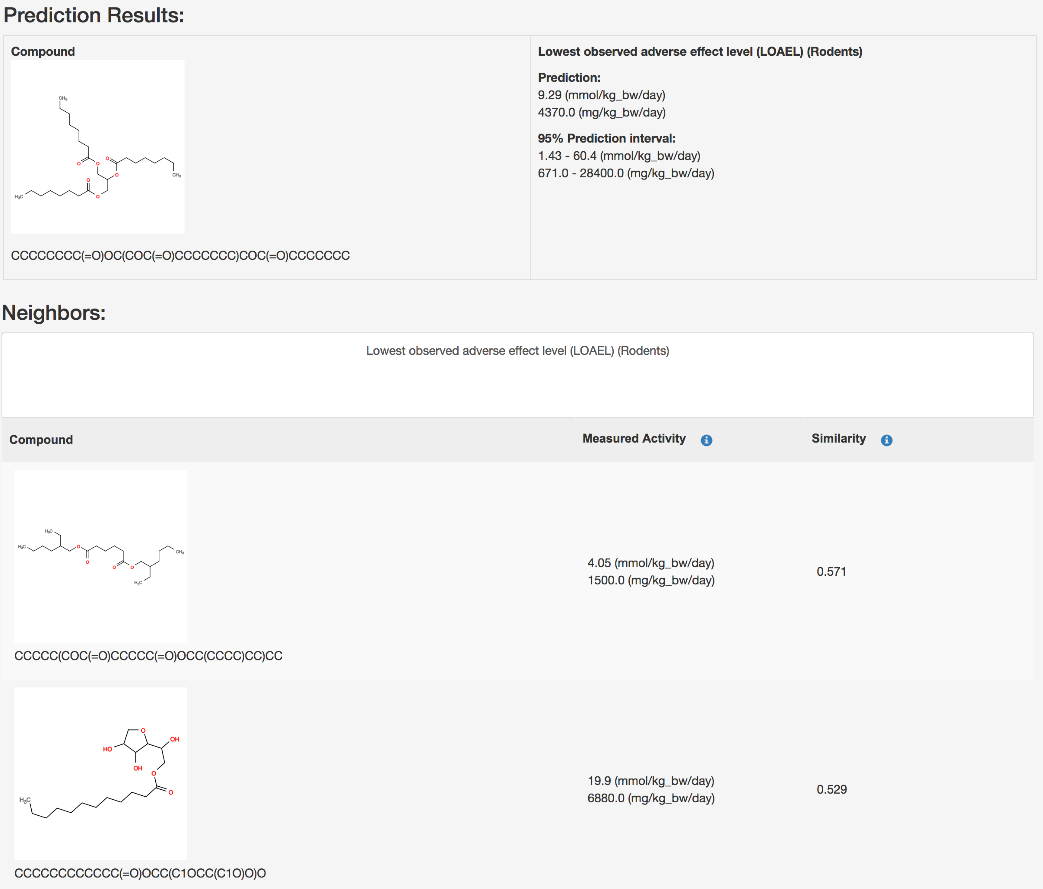
\includegraphics{figures/lazar-screenshot.pdf}
\caption{Screenshot of a lazar prediction from the public
webinterface.}\label{fig:screenshot}
\end{figure}

\section{Results}\label{results}

\subsubsection{Dataset comparison}\label{dataset-comparison}

The main objective of this section is to compare the content of both
databases in terms of structural composition and LOAEL values, to
estimate the experimental variability of LOAEL values and to establish a
baseline for evaluating prediction performance.

\subparagraph{Structural diversity}\label{structural-diversity}

In order to compare the structural diversity of both databases we
evaluated the frequency of functional groups from the OpenBabel FP4
fingerprint. Figure~\ref{fig:fg} shows the frequency of functional
groups in both databases. 139 functional groups with a frequency
\textgreater{} 25 are depicted, the complete table for all functional
groups can be found in the supplemental material at
\href{https://github.com/opentox/loael-paper/blob/revision/data/functional-groups.csv}{GitHub}.

\begin{figure}
\centering
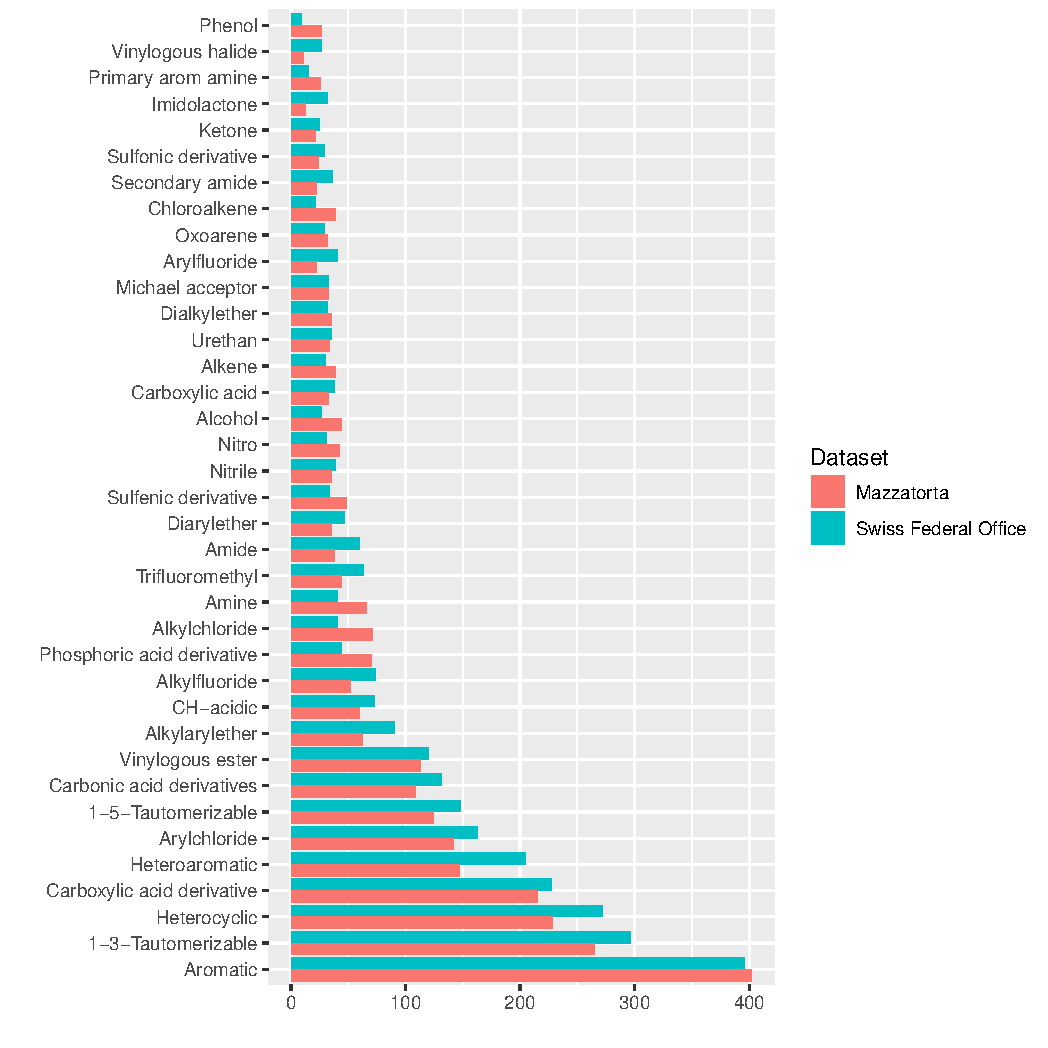
\includegraphics{figures/functional-groups.pdf}
\caption{Frequency of functional groups.}\label{fig:fg}
\end{figure}

This result was confirmed with a visual inspection using the
\href{http://ches-mapper.org}{CheS-Mapper} (Chemical Space Mapping and
Visualization in 3D, Gütlein, Karwath, and Kramer (2012)) tool.
CheS-Mapper can be used to analyze the relationship between the
structure of chemical compounds, their physico-chemical properties, and
biological or toxic effects. It depicts closely related (similar)
compounds in 3D space and can be used with different kinds of features.
We have investigated structural as well as physico-chemical properties
and concluded that both databases are very similar, both in terms of
chemical structures and physico-chemical properties.

The only statistically significant difference between both databases is
that the Nestlé database contains more small compounds (61 structures
with less than 11 non-hydrogen atoms) than the FSVO-database (19 small
structures, chi-square test: p-value 3.7E-7).

\subsubsection{Experimental variability versus prediction
uncertainty}\label{experimental-variability-versus-prediction-uncertainty}

Duplicated LOAEL values can be found in both databases and there is a
substantial number of 155 compounds with more than one LOAEL. These
chemicals allow us to estimate the variability of experimental results
within individual databases and between databases. Data with
\emph{identical} values (at five significant digits) in both databases
were excluded from variability analysis, because it it likely that they
originate from the same experiments.

\subparagraph{Intra database
variability}\label{intra-database-variability}

Both databases contain substances with multiple measurements, which
allow the determination of experimental variabilities. For this purpose
we have calculated the mean LOAEL standard deviation of compounds with
multiple measurements. Mean standard deviations and thus experimental
variabilities are similar for both databases.

The Nestlé database has 567 LOAEL values for 445 unique structures, 93
compounds have multiple measurements with a mean standard deviation
(-log10 transformed values) of 0.32 (0.56 mg/kg\_bw/day, 0.56
mmol/kg\_bw/day) (P. Mazzatorta et al. (2008), Figure~\ref{fig:intra}).

The FSVO database has 493 rat LOAEL values for 381 unique structures, 91
compounds have multiple measurements with a mean standard deviation
(-log10 transformed values) of 0.29 (0.57 mg/kg\_bw/day, 0.59
mmol/kg\_bw/day) (Figure~\ref{fig:intra}).

Standard deviations of both databases do not show a statistically
significant difference with a p-value (t-test) of 0.21. The combined
test set has a mean standard deviation (-log10 transformed values) of
0.33 (0.56 mg/kg\_bw/day, 0.55 mmol/kg\_bw/day)
(Figure~\ref{fig:intra}).

\begin{figure}
\centering
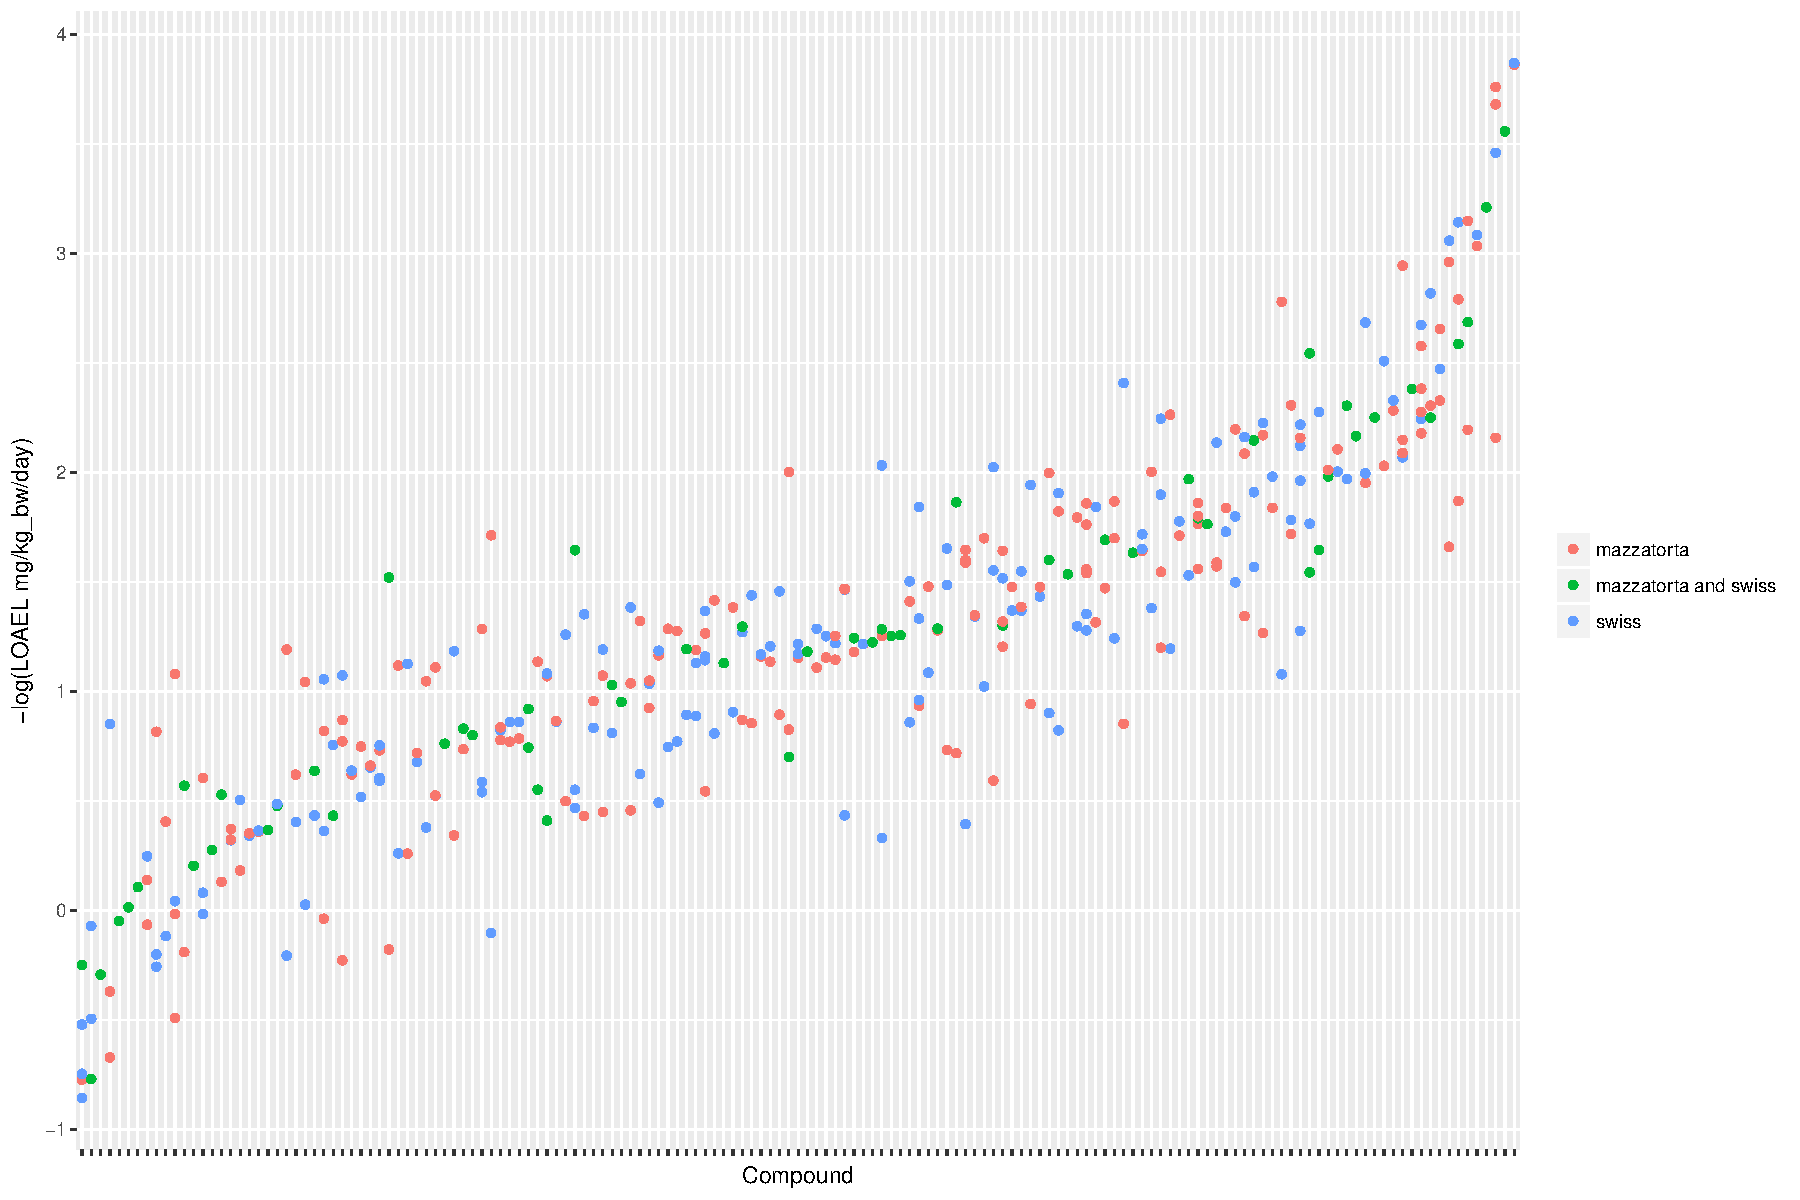
\includegraphics{figures/dataset-variability.pdf}
\caption{LOAEL distribution and variability of compounds with multiple
measurements in both databases. Compounds were sorted according to LOAEL
values. Each vertical line represents a compound, and each dot an
individual LOAEL value. Experimental variability can be inferred from
dots (LOAELs) on the same line (compound).}\label{fig:intra}
\end{figure}

\subparagraph{Inter database
variability}\label{inter-database-variability}

In order to compare the correlation of LOAEL values in both databases
and to establish a reference for predicted values, we have investigated
compounds, that occur in both databases.

Figure~\ref{fig:datacorr} depicts the correlation between LOAEL values
from both databases. As both databases contain duplicates medians were
used for the correlation plot and statistics. It should be kept in mind
that the aggregation of duplicated measurements into a single median
value hides a substantial portion of the experimental variability.
Correlation analysis shows a significant (p-value \textless{} 2.2e-16)
correlation between the experimental data in both databases with r\^{}2:
0.52, RMSE: 0.59

Figure~\ref{fig:comp} shows the experimental LOAEL variability of
compounds occurring in both datasets (i.e.~the \emph{test} dataset)
colored in blue (experimental). This is the baseline reference for the
comparison with predicted values.

\begin{figure}
\centering
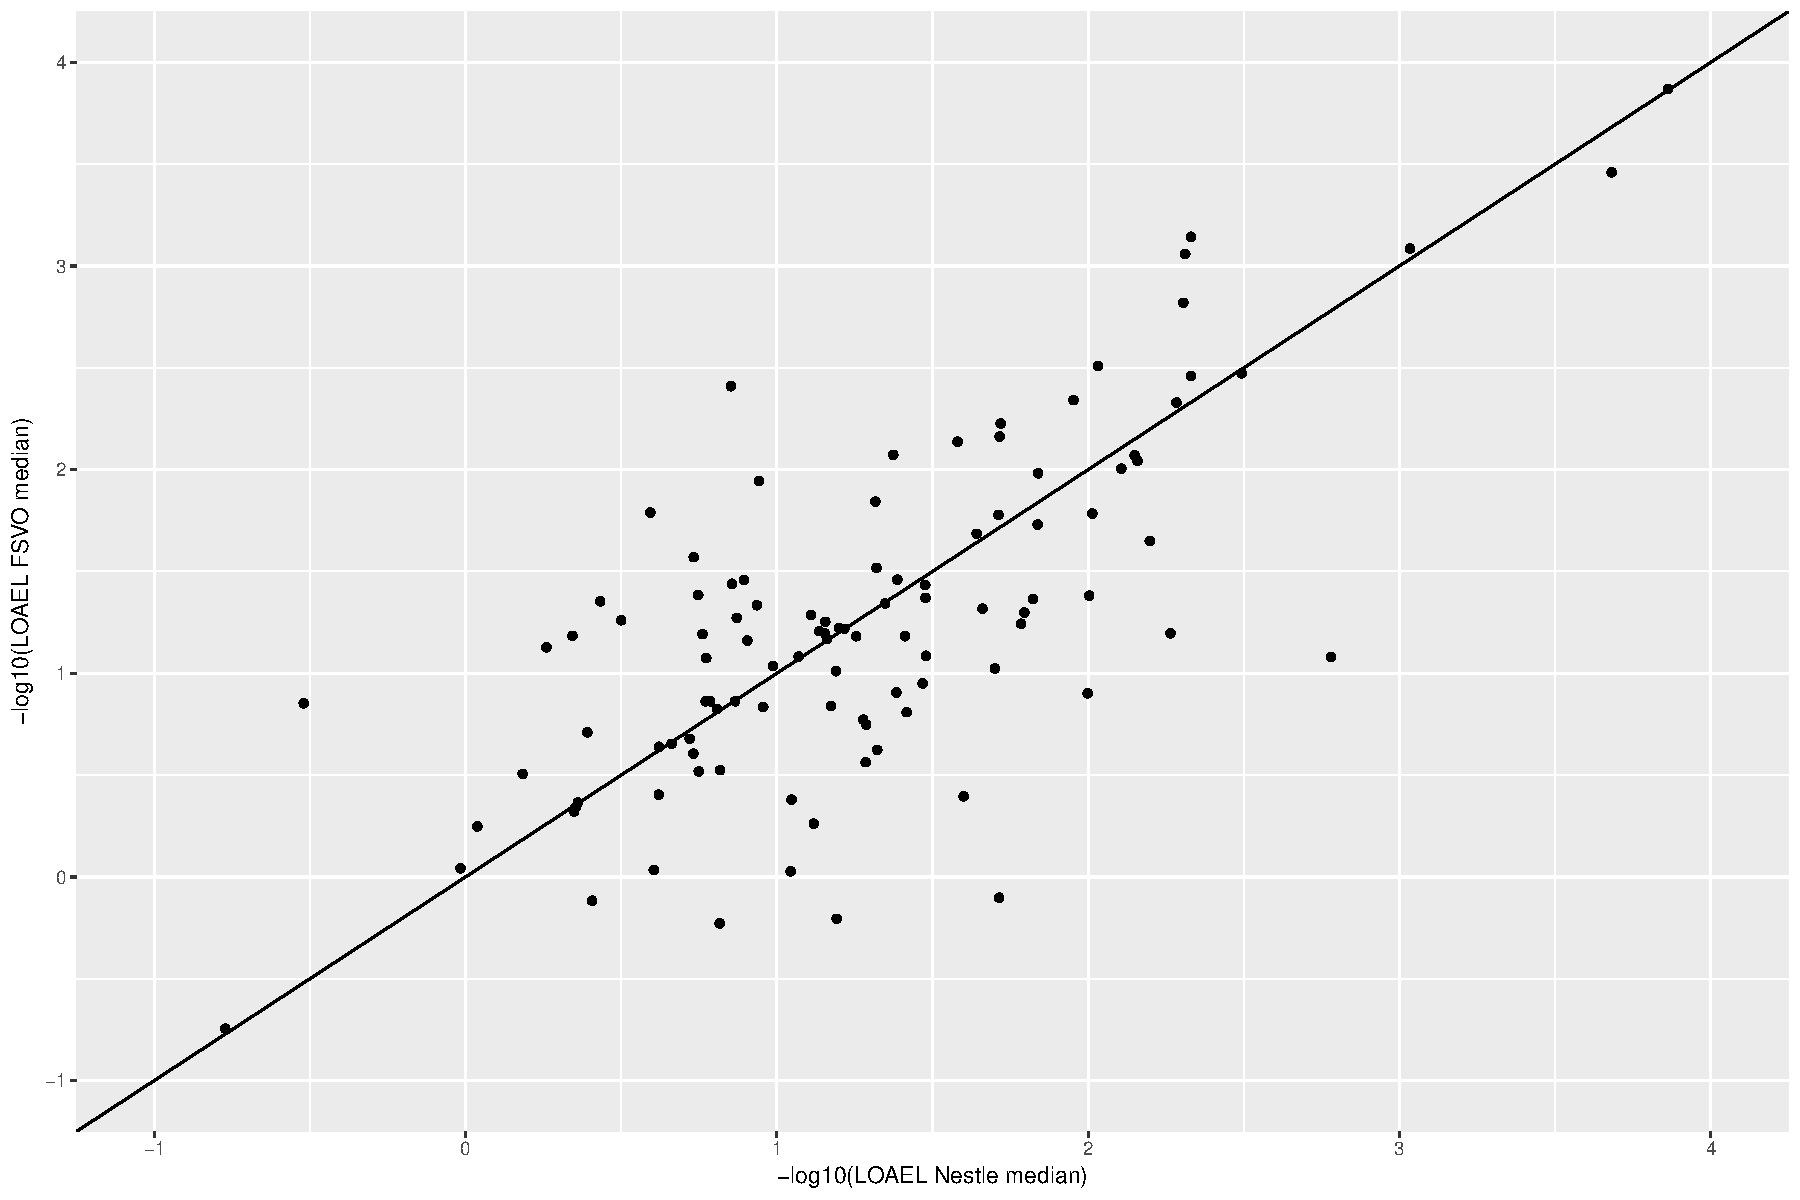
\includegraphics{figures/median-correlation.pdf}
\caption{Correlation of median LOAEL values from Nestlé and FSVO
databases. Data with identical values in both databases was removed from
analysis.}\label{fig:datacorr}
\end{figure}

\subsubsection{Local QSAR models}\label{local-qsar-models}

In order to compare the performance of \emph{in silico} read across
models with experimental variability we used compounds with multiple
measurements as a test set (375 measurements, 155 compounds).
\texttt{lazar} read across predictions were obtained for 155 compounds,
37 predictions failed, because no similar compounds were found in the
training data (i.e.~they were not covered by the applicability domain of
the training data).

In 100\% of the test examples experimental LOAEL values were located
within the 95\% prediction intervals.

Figure~\ref{fig:comp} shows a comparison of predicted with experimental
values. Most predicted values were located within the experimental
variability.

\begin{figure}
\centering
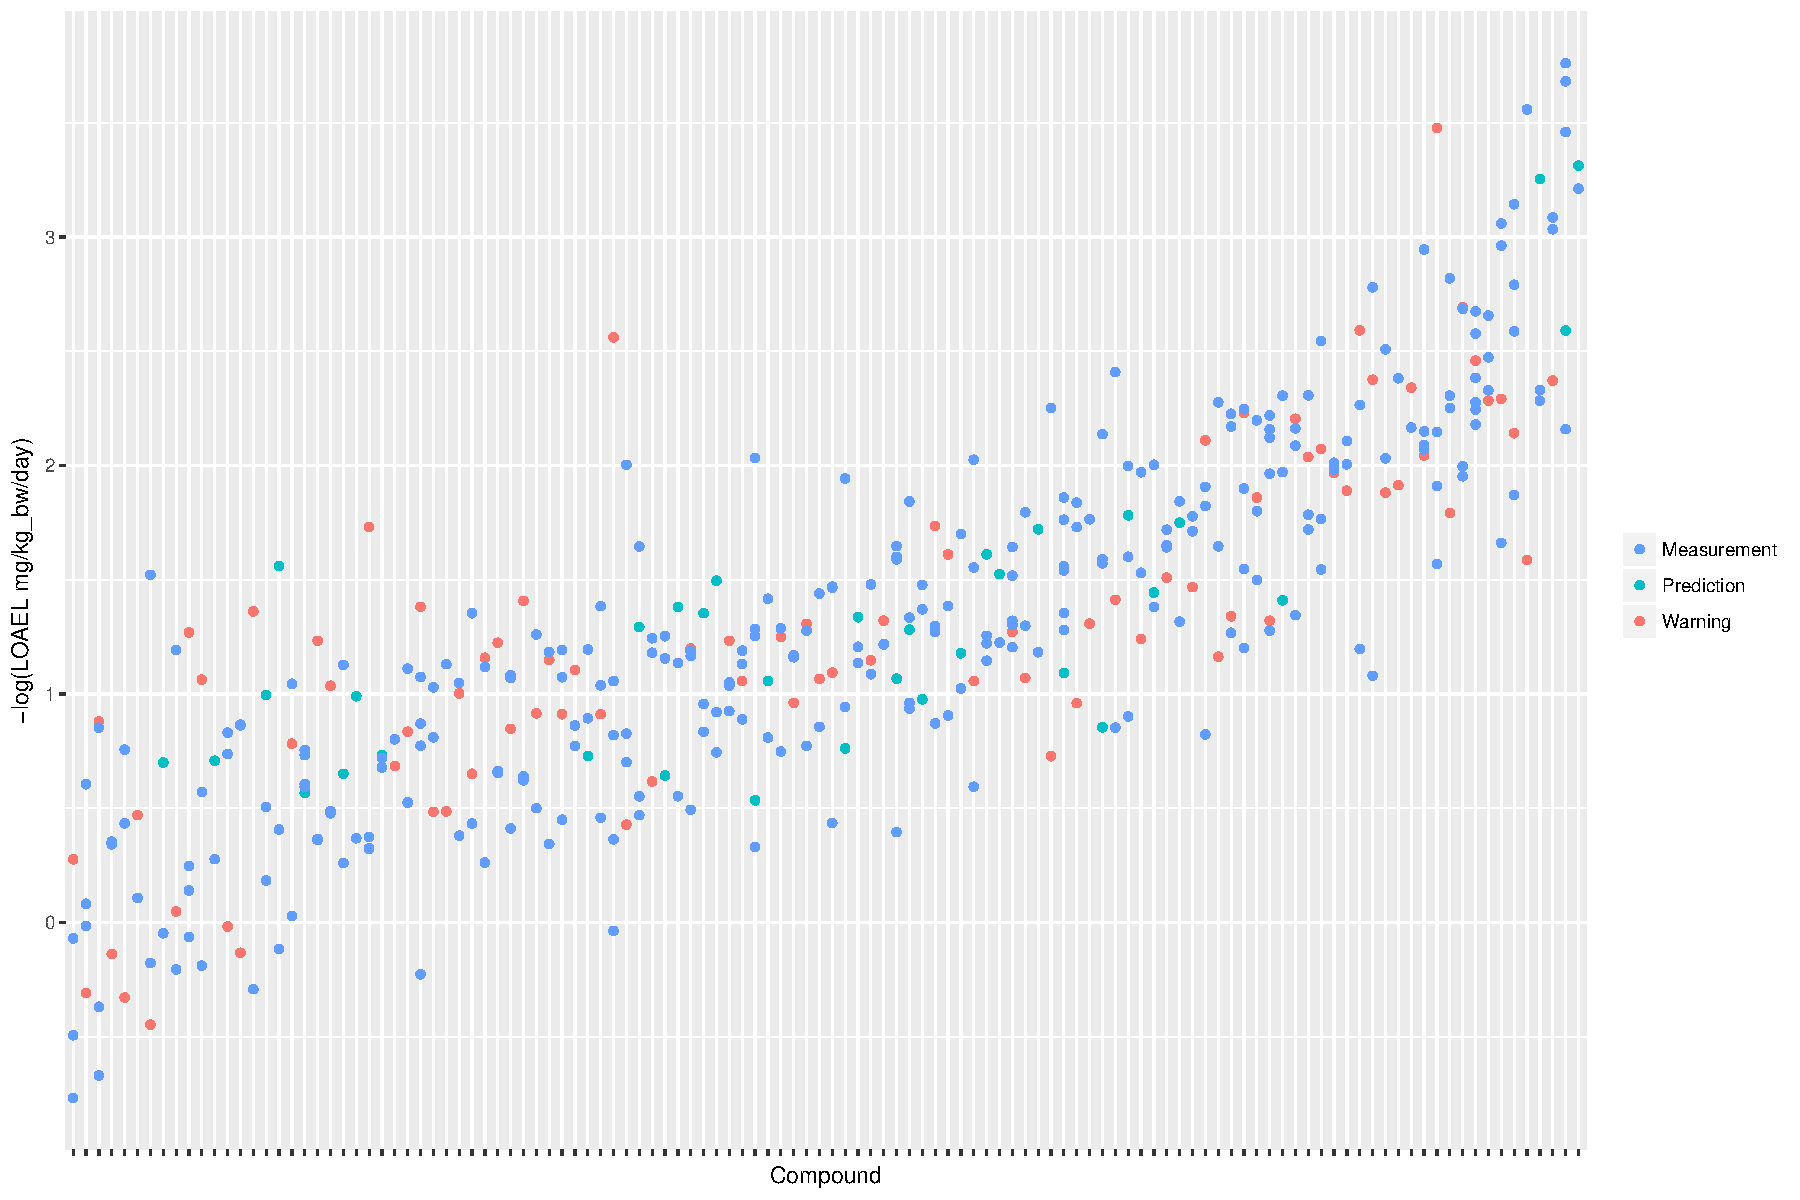
\includegraphics{figures/test-prediction.pdf}
\caption{Comparison of experimental with predicted LOAEL values. Each
vertical line represents a compound, dots are individual measurements
(blue), predictions (green) or predictions far from the applicability
domain, i.e.~with warnings (red).}\label{fig:comp}
\end{figure}

Correlation analysis was performed between individual predictions and
the median of experimental data. All correlations are statistically
highly significant with a p-value \textless{} 2.2e-16. These results are
presented in Figure~\ref{fig:corr} and Table~\ref{tbl:cv}. Please bear
in mind that the aggregation of multiple measurements into a single
median value hides experimental variability.

\hypertarget{tbl:common-pred}{}
\begin{longtable}[]{@{}llll@{}}
\caption{\label{tbl:common-pred}Comparison of model predictions with
experimental variability. }\tabularnewline
\toprule
Comparison & \(r^2\) & RMSE & Nr. predicted\tabularnewline
\midrule
\endfirsthead
\toprule
Comparison & \(r^2\) & RMSE & Nr. predicted\tabularnewline
\midrule
\endhead
Nestlé vs.~FSVO database & 0.52 & 0.59\tabularnewline
AD close predictions vs.~test median & 0.48 & 0.56 &
34/155\tabularnewline
AD distant predictions vs.~test median & 0.38 & 0.68 &
84/155\tabularnewline
All predictions vs.~test median & 0.4 & 0.65 & 118/155\tabularnewline
\bottomrule
\end{longtable}

\begin{figure}
\centering
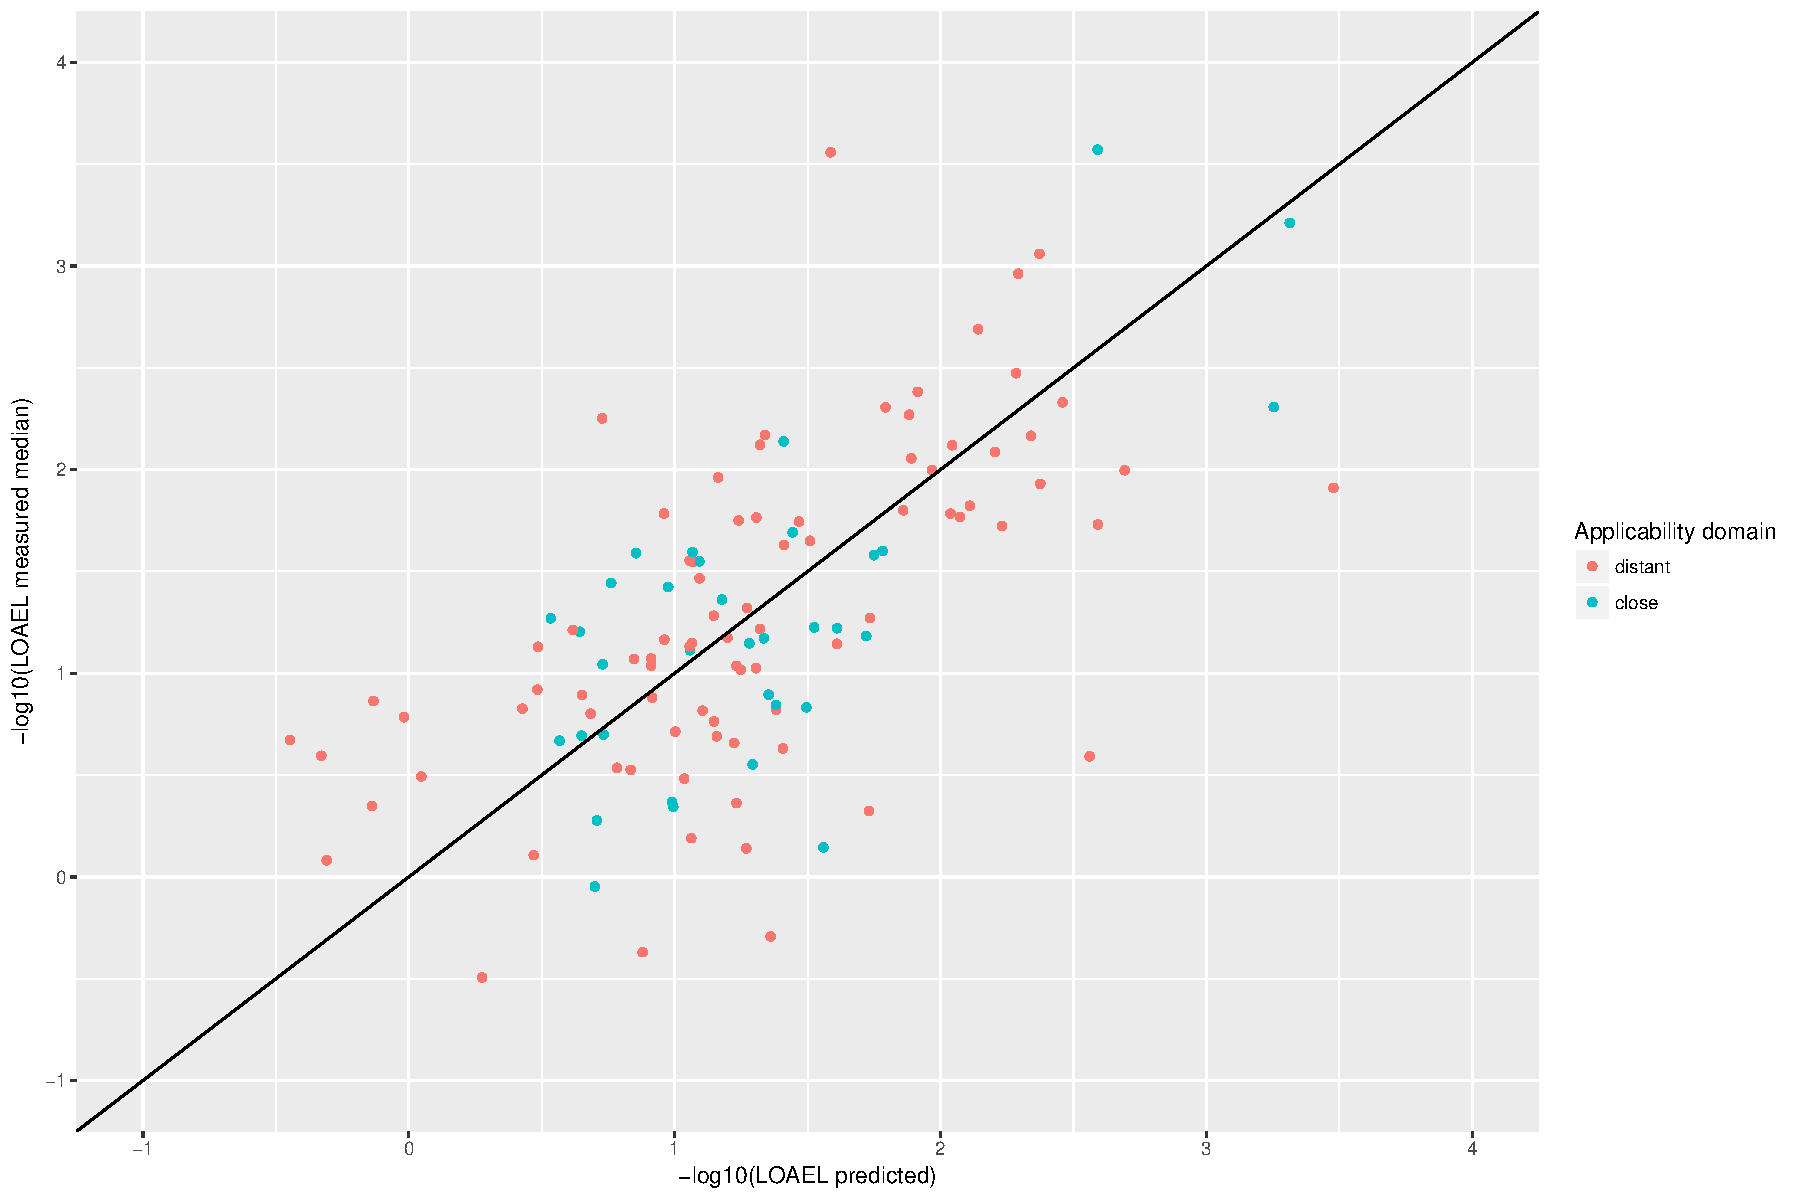
\includegraphics{figures/prediction-test-correlation.pdf}
\caption{Correlation of experimental with predicted LOAEL values (test
set). Green dots indicate predictions close to the applicability domain
(i.e.~without warnings), red dots indicate predictions far from the
applicability domain (i.e.~with warnings).}\label{fig:corr}
\end{figure}

For a further assessment of model performance three independent 10-fold
cross-validations were performed. Results are summarised in
Table~\ref{tbl:cv} and Figure~\ref{fig:cv}. All correlations of
predicted with experimental values are statistically highly significant
with a p-value \textless{} 2.2e-16. This was observed for compounds
close and more distant to the applicability domain.

\hypertarget{tbl:cv}{}
\begin{longtable}[]{@{}llll@{}}
\caption{\label{tbl:cv}Results (mean and standard deviation) from 50
independent 10-fold crossvalidations }\tabularnewline
\toprule
Predictions & \(r^2\) & RMSE & Nr. predicted\tabularnewline
\midrule
\endfirsthead
\toprule
Predictions & \(r^2\) & RMSE & Nr. predicted\tabularnewline
\midrule
\endhead
AD close & 0.6 \(\pm\) 0.04 & 0.58 \(\pm\) 0.02 & 97 \(\pm\)
4\tabularnewline
AD distant & 0.43 \(\pm\) 0.01 & 0.8 \(\pm\) 0.01 & 380 \(\pm\)
5\tabularnewline
All & 0.46 \(\pm\) 0.01 & 0.76 \(\pm\) 0.01 & 477 \(\pm\)
4\tabularnewline
\bottomrule
\end{longtable}

\begin{figure}
\centering
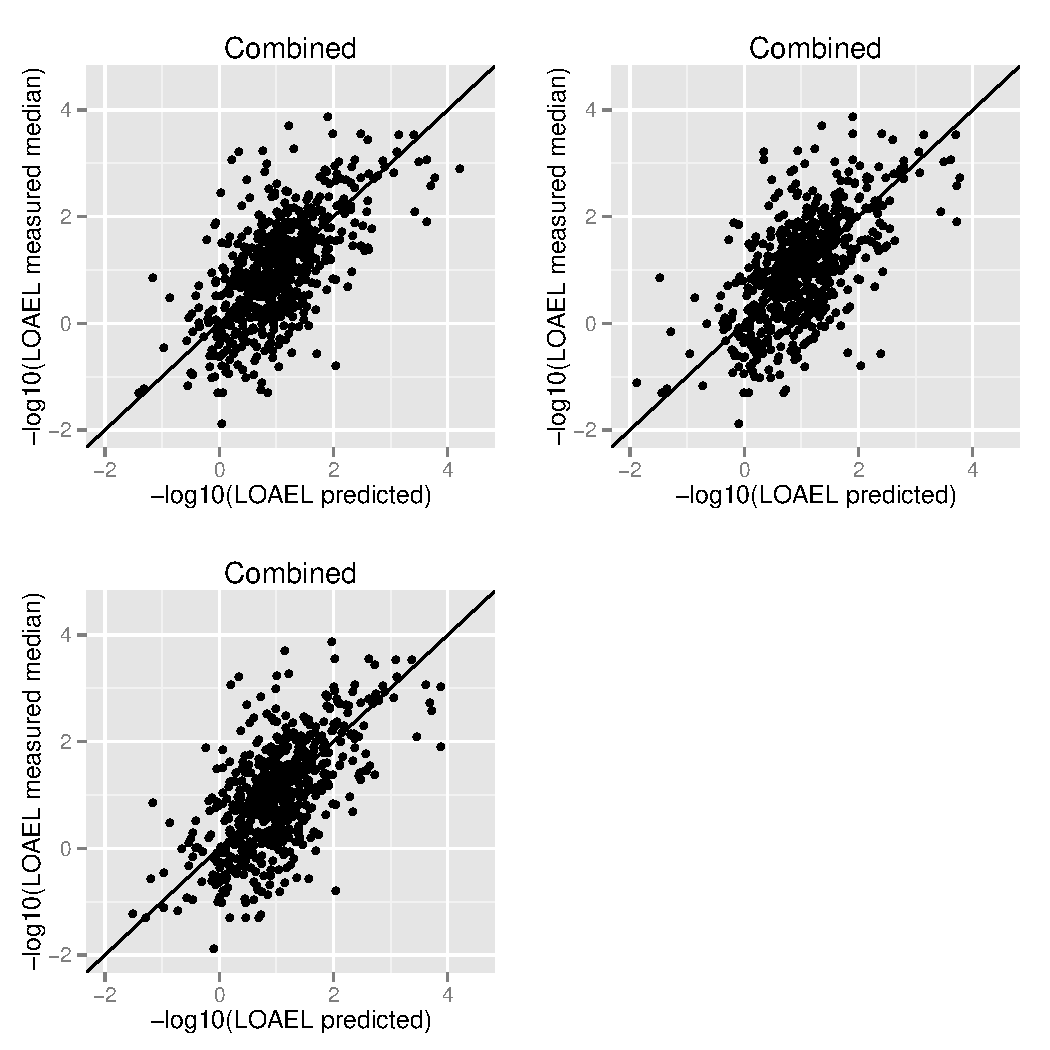
\includegraphics{figures/crossvalidation.pdf}
\caption{Correlation of predicted vs.~measured values from a randomly
selected crossvalidation with MP2D fingerprint descriptors and local
random forest models.}\label{fig:cv}
\end{figure}

\section{Discussion}\label{discussion}

It is currently acknowledged that there is a strong need for
toxicological information on the multiple thousands of chemicals to
which human may be exposed through food. These include for example many
chemicals in commerce, which could potentially find their way into food
(Stanton and Krusezewski 2016, Fowler, Savage, and Mendez (2011)), but
also substances migrating from food contact materials (Grob et al.
2006), chemicals generated over food processing (Cotterill et al. 2008),
environmental contaminants as well as inherent plant toxicants
(Schilter, Constable, and Perrin 2013). For the vast majority of these
chemicals, no toxicological data is available and consequently insight
on their potential health risks is very difficult to obtain. It is
recognized that testing all of them in standard animal studies is
neither feasible from a resource perspective nor desirable because of
ethical issues associated with animal experimentation. In addition, for
many of these chemicals, risk may be very low and therefore testing may
actually be irrelevant. In this context, the identification of chemicals
of most concern on which limited resource available should focused is
essential and computational toxicology is thought to play an important
role for that.

In order to establish the level of safety concern of food chemicals
toxicologically not characterized, a methodology mimicking the process
of chemical risk assessment, and supported by computational toxicology,
was proposed (Schilter et al. 2014). It is based on the calculation of
margins of exposure (MoE) that is the ratio between the predicted
chronic toxicity value (LOAEL) and exposure estimate. The level of
safety concern of a chemical is then determined by the size of the MoE
and its suitability to cover the uncertainties of the assessment. To be
applicable, such an approach requires quantitative predictions of
toxicological endpoints relevant for risk assessment. The present work
focuses on the prediction of chronic toxicity, a major and often pivotal
endpoint of toxicological databases used for hazard identification and
characterization of food chemicals.

In a previous study, automated read-across like models for predicting
carcinogenic potency were developed. In these models, substances in the
training dataset similar to the query compounds are automatically
identified and used to derive a quantitative TD50 value. The errors
observed in these models were within the published estimation of
experimental variability (Lo Piparo et al. 2014). In the present study,
a similar approach was applied to build models generating quantitative
predictions of long-term toxicity. Two databases compiling chronic oral
rat lowest adverse effect levels (LOAEL) as reference value were
available from different sources. Our investigations clearly indicated
that the Nestlé and FSVO databases are very similar in terms of chemical
structures and properties as well as distribution of experimental LOAEL
values. The only significant difference that we observed was that the
Nestlé one has larger amount of small molecules, than the FSVO database.
For this reason we pooled both databases into a single training dataset
for read across predictions.

An early review of the databases revealed that 155 out of the 671
chemicals available in the training datasets had at least two
independent studies/LOAELs. These studies were exploited to generate
information on the reproducibility of chronic animal studies and were
used to evaluate prediction performance of the models in the context of
experimental variability. Considerable variability in the experimental
data was observed. Study design differences, including dose selection,
dose spacing and route of administration are likely explanation of
experimental variability. High experimental variability has an impact on
model building and on model validation. First it influences model
quality by introducing noise into the training data, secondly it
influences accuracy estimates because predictions have to be compared
against noisy data where ``true'' experimental values are unknown. This
will become obvious in the next section, where comparison of predictions
with experimental data is discussed. The data obtained in the present
study indicate that \texttt{lazar} generates reliable predictions for
compounds within the applicability domain of the training data
(i.e.~predictions without warnings, which indicates a sufficient number
of neighbors with similarity \textgreater{} 0.5 to create local random
forest models). Correlation analysis shows that errors (\(\text{RMSE}\))
and explained variance (\(r^{2}\)) are comparable to experimental
variability of the training data.

Predictions with a warning (neighbor similarity \textless{} 0.5 and
\textgreater{} 0.2 or weighted average predictions) are more uncertain.
However, they still show a strong correlation with experimental data,
but the errors are \textasciitilde{} 20-40\% larger than for compounds
within the applicability domain (Figure~\ref{fig:corr} and
Table~\ref{tbl:cv}). Expected errors are displayed as 95\% prediction
intervals, which covers 100\% of the experimental data. The main
advantage of lowering the similarity threshold is that it allows to
predict a much larger number of substances than with more rigorous
applicability domain criteria. As each of this prediction could be
problematic, they are flagged with a warning to alert risk assessors
that further inspection is required. This can be done in the graphical
interface (\url{https://lazar.in-silico.ch}) which provides intuitive
means of inspecting the rationales and data used for read across
predictions.

Finally there is a substantial number of chemicals (37), where no
predictions can be made, because no similar compounds in the training
data are available. These compounds clearly fall beyond the
applicability domain of the training dataset and in such cases
predictions should not be used. In order to expand the domain of
applicability, the possibility to design models based on shorter, less
than chonic studies should be studied. It is likely that more substances
reflecting a wider chemical domain may be available. To predict such
shorter duration endpoints would also be valuable for chronic toxicy
since evidence suggest that exposure duration has little impact on the
levels of NOAELs/LOAELs (Zarn, Engeli, and Schlatter 2011, Zarn, Engeli,
and Schlatter (2013)).

\subsubsection{\texorpdfstring{\texttt{lazar}
predictions}{lazar predictions}}\label{lazar-predictions}

Table~\ref{tbl:common-pred}, Table~\ref{tbl:cv}, Figure~\ref{fig:comp},
Figure~\ref{fig:corr} and Figure~\ref{fig:cv} clearly indicate that
\texttt{lazar} generates reliable predictions for compounds within the
applicability domain of the training data (i.e.~predictions without
warnings, which indicates a sufficient number of neighbors with
similarity \textgreater{} 0.5 to create local random forest models).
Correlation analysis (Table~\ref{tbl:common-pred}, Table~\ref{tbl:cv})
shows, that errors (\(RMSE\)) and explained variance (\(r^2\)) are
comparable to experimental variability of the training data.

Predictions with a warning (neighbor similarity \textless{} 0.5 and
\textgreater{} 0.2 or weighted average predictions) are a grey zone.
They still show a strong correlation with experimental data, but the
errors are larger than for compounds within the applicability domain
(Table~\ref{tbl:common-pred}, Table~\ref{tbl:cv}). Expected errors are
displayed as 95\% prediction intervals, which covers 100\% of the
experimental data. The main advantage of lowering the similarity
threshold is that it allows to predict a much larger number of
substances than with more rigorous applicability domain criteria. As
each of this prediction could be problematic, they are flagged with a
warning to alert risk assessors that further inspection is required.
This can be done in the graphical interface
(\url{https://lazar.in-silico.ch}) which provides intuitive means of
inspecting the rationales and data used for read across predictions.

\section{Summary}\label{summary}

In conclusion, we could demonstrate that \texttt{lazar} predictions
within the applicability domain of the training data have the same
variability as the experimental training data. In such cases
experimental investigations can be substituted with \emph{in silico}
predictions. Predictions with a lower similarity threshold can still
give usable results, but the errors to be expected are higher and a
manual inspection of prediction results is highly recommended. Anyway,
our suggested workflow includes always the visual inspection of the
chemical structures of the neighbors selected by the model. Indeed it
will strength the prediction confidence (if the input structure looks
very similar to the neighbors selected to build the model) or it can
drive to the conclusion to use read-across with the most similar
compound of the database (in case not enough similar compounds to build
the model are present in the database).

\section*{References}\label{references}
\addcontentsline{toc}{section}{References}

\hypertarget{refs}{}
\hypertarget{ref-doi:10.1021ux2fci034207y}{}
Bender, Andreas, Hamse Y. Mussa, Robert C. Glen, and Stephan Reiling.
2004. ``Molecular Similarity Searching Using Atom Environments,
Information-Based Feature Selection, and a Naïve Bayesian Classifier.''
\emph{Journal of Chemical Information and Computer Sciences} 44 (1):
170--78.
doi:\href{https://doi.org/10.1021/ci034207y}{10.1021/ci034207y}.

\hypertarget{ref-Cotterill2008}{}
Cotterill, J.V., M.Q. Chaudry, W. Mattews, and R. W. Watkins. 2008. ``In
Silico Assessment of Toxicity of Heat-Generated Food Contaminants.''
\emph{Food Chemical Toxicology}, no. 46(6): 1905--18.

\hypertarget{ref-ECHA2008}{}
ECHA. 2008. ``Guidance on Information Requirements and Chemical Safety
Assessment, Chapter R.6: QSARs and Grouping of Chemicals.'' ECHA.

\hypertarget{ref-EFSA2014}{}
EFSA. 2014. ``Rapporteur Member State Assessment Reports Submitted for
the EU Peer Review of Active Substances Used in Plant Protection
Products.'' \url{http://dar.efsa.europa.eu/dar-web/provision}.

\hypertarget{ref-EFSA2016}{}
EFSA. 2016. ``Guidance on the Establishment of the Residue Definition
for Dietary Assessment: EFSA Panel on Plant Protect Products and Their
Residues (PPR).'' \emph{EFSA Journal}, no. 14: 1--12.

\hypertarget{ref-Fowler2011}{}
Fowler, B., S. Savage, and B. Mendez. 2011. ``White Paper: Protecting
Public Health in the 21st Century: The Case for Computational
Toxicology.'' ICF International, Inc.icfi.com.

\hypertarget{ref-Grob2006}{}
Grob, K., M. Biedermann, E. Scherbaum, M. Roth, and K. Rieger. 2006.
``Food Contamination with Organic Materials in Perspective: Packaging
Materials as the Largest and Least Controlled Source? A View Focusing on
the European Situation.'' \emph{Crit. Rev. Food. Sci. Nutr.}, no. 46:
529--35.
doi:\href{https://doi.org/10.1080/10408390500295490}{10.1080/10408390500295490}.

\hypertarget{ref-Guetlein2012}{}
Gütlein, Martin, Andreas Karwath, and Stefan Kramer. 2012. ``CheS-Mapper
- Chemical Space Mapping and Visualization in 3D.'' \emph{Journal of
Cheminformatics} 4 (1): 7.
doi:\href{https://doi.org/10.1186/1758-2946-4-7}{10.1186/1758-2946-4-7}.

\hypertarget{ref-HealthCanada2016}{}
Health Canada. 2016.
\url{https://www.canada.ca/en/health-canada/services/chemical-substances/chemicals-management-plan.html}.

\hypertarget{ref-Kuhn08}{}
Kuhn, Max. 2008. ``Building Predictive Models in R Using the Caret
Package.'' \emph{J. of Stat. Soft}.

\hypertarget{ref-LoPiparo2014}{}
Lo Piparo, E., A. Maunz, C. Helma, D. Vorgrimmler, and B. Schilter.
2014. ``Automated and Reproducible Read-Across Like Models for
Predicting Carcinogenic Potency.'' \emph{Regulatory Toxicology and
Pharmacology}, no. 70: 370--78.

\hypertarget{ref-LoPiparo2011}{}
Lo Piparo, E., A. Worth, A. Manibusan, C. Yang, B. Schilter, P.
Mazzatorta, M.N. Jacobs, H. Steinkelner, and L. Mohimont. 2011. ``Use of
Computational Tools in the Field of Food Safety.'' \emph{Regulatory
Toxicology and Pharmacology}, no. 60(3): 354--62.

\hypertarget{ref-Maunz2013}{}
Maunz, Andreas, Martin Gütlein, Micha Rautenberg, David Vorgrimmler,
Denis Gebele, and Christoph Helma. 2013. ``Lazar: A Modular Predictive
Toxicology Framework.'' \emph{Frontiers in Pharmacology} 4. Frontiers
Media SA.
doi:\href{https://doi.org/10.3389/fphar.2013.00038}{10.3389/fphar.2013.00038}.

\hypertarget{ref-mazzatorta08}{}
Mazzatorta, Paolo, Manuel Dominguez Estevez, Myriam Coulet, and Benoit
Schilter. 2008. ``Modeling Oral Rat Chronic Toxicity.'' \emph{Journal of
Chemical Information and Modeling} 48 (10): 1949--54.
doi:\href{https://doi.org/10.1021/ci8001974}{10.1021/ci8001974}.

\hypertarget{ref-OBoyle2011}{}
OBoyle, Noel M, Michael Banck, Craig A James, Chris Morley, Tim
Vandermeersch, and Geoffrey R Hutchison. 2011. ``Open Babel: An Open
Chemical Toolbox.'' \emph{Journal of Cheminformatics} 3 (1). Springer
Science and Business Media: 33.
doi:\href{https://doi.org/10.1186/1758-2946-3-33}{10.1186/1758-2946-3-33}.

\hypertarget{ref-OECD2015}{}
OECD. 2015. ``Fundamental and Guiding Principles for (Q)SAR Analysis of
Chemicals Carcinogens with Mechanistic Considerations Monograph 229
ENV/JM/MONO(2015)46.'' In \emph{Series on Testing and Assessment No
229}.

\hypertarget{ref-Schilter2014}{}
Schilter, B., R. Benigni, A. Boobis, A. Chiodini, A. Cockburn, M.T.
Cronin, E. Lo Piparo, S. Modi, Thiel A., and A. Worth. 2014.
``Establishing the Level of Safety Concern for Chemicals in Food Without
the Need for Toxicity Testing.'' \emph{Regulatory Toxicology and
Pharmacology}, no. 68: 275--98.

\hypertarget{ref-Schilter2013}{}
Schilter, B., A. Constable, and I. Perrin. 2013. ``Naturally Occurring
Toxicants of Plant Origin: Risk Assessment and Management
Considerations.'' In \emph{Food Safety Management: A Practical Guide for
Industry}, edited by Y. Motarjemi, 45--57. Elsevier.

\hypertarget{ref-Stanton2016}{}
Stanton, K., and F.H. Krusezewski. 2016. ``Quantifying the Benefits of
Using Read-Across and in Silico Techniques to Fullfill Hazard Data
Requirements for Chemical Categories.'' \emph{Regulatory Toxicology and
Pharmacology}, no. 81: 250--59.
doi:\href{https://doi.org/10.1016/j-yrtph.2016.09.004.}{10.1016/j-yrtph.2016.09.004.}

\hypertarget{ref-EPA2011}{}
US EPA. 2011. ``Fact Sheets on New Active Ingredients.''

\hypertarget{ref-doi:10.1021ux2fci00057a005}{}
Weininger, David. 1988. ``SMILES, a Chemical Language and Information
System. 1. Introduction to Methodology and Encoding Rules.''
\emph{Journal of Chemical Information and Computer Sciences} 28 (1):
31--36.
doi:\href{https://doi.org/10.1021/ci00057a005}{10.1021/ci00057a005}.

\hypertarget{ref-WHO2011}{}
WHO. 2011. ``Joint FAO/WHO Meeting on Pesticide Residues (JMPR)
Publications.''
\url{http://www.who.int/foodsafety/publications/jmpr-monographs/en/}.

\hypertarget{ref-Zarn2011}{}
Zarn, J.A., B.E. Engeli, and J.R. Schlatter. 2011. ``Study Parameters
Influencing NOAEL and LOAEL in Toxicity Feeding Studies for Pesticides:
Exposure Duration Versus Dose Decrement, Dose Spacing, Group Size and
Chemical Class.'' \emph{Regul. Toxicol. Pharmacol.}, no. 61: 243--50.

\hypertarget{ref-Zarn2013}{}
---------. 2013. ``Characterization of the Dose Decrement in Regulatory
Rat Pesticide Toxicity Feeding Studies.'' \emph{Regul. Toxicol.
Pharmacol.}, no. 67: 215--20.

\end{document}
